\documentclass{article}

% Taille exacte
\newcommand{\bigtext}{\fontsize{16pt}{20pt}\selectfont}
\newcommand{\smalltext}{\fontsize{12pt}{16pt}\selectfont}

% =====================
% ENCODAGE & LANGUE
% =====================
\usepackage[utf8]{inputenc}
\usepackage[french]{babel}

% =====================
% PACKAGES GÉNÉRAUX
% =====================
\usepackage{amsmath, amsthm, amsfonts, amssymb}
\usepackage{hyperref}
\usepackage{url}
\usepackage{listings}
\usepackage{color}
\usepackage[tikz]{bclogo}
\usepackage{tcolorbox}
\usepackage{fancyhdr}
\usepackage{geometry}
\usepackage{graphicx}
\usepackage{alltt}

%\sloppy

% =====================
% CONFIGURATION DU CODE
% =====================
\lstset{
   breaklines=true,        % autorise la coupure automatique
  language=java,
  escapeinside={@*}{*@},
  %basicstyle=\ttfamily
}

\newcommand{\code}[1]{\lstinline{#1}}

% =====================
% MISE EN PAGE
% =====================
\geometry{a4paper, margin=1in}
\fancyhf{}
\fancyhead[L]{Université de Bordeaux -- Département Informatique -- Master}
\fancyhead[R]{4TIN706U Approche Objet}
\fancyfoot[C]{\thepage}
\pagestyle{fancy}

% =====================
% BOÎTES & EN-TÊTES
% =====================
\newcommand{\CMheader}[1]{
    \begin{tcolorbox}[colback=gray!10!white, colframe=gray!80!black, width=\textwidth, sharp corners]
        \centering
        \vspace{0.2cm}
        \textbf{#1}
    \end{tcolorbox}
}

\newcommand{\TDheader}[2]{
    \renewcommand{\TDNum}{#2}
    \begin{tcolorbox}[colback=gray!10!white, colframe=gray!80!black, width=\textwidth, sharp corners]
        \centering
        \vspace{0.2cm}
        \textbf{\Large TD N\textsuperscript{o}#2} \\
        \textbf{#1}
    \end{tcolorbox}
}

\newcommand{\PROJECTheader}[1]{
    \begin{tcolorbox}[colback=gray!10!white, colframe=gray!80!black, width=\textwidth, sharp corners]
        \centering
        \vspace{0.2cm}
        \textbf{\Large Projet} \\
        \textbf{#1}
    \end{tcolorbox}
}

\begin{document}
%\bigtext

\PROJECTheader{Mazing: une API graphique pour jeu d'aventure en projection isométrique}

\section*{Introduction}

\textbf{Mazing} est une API Java qui exploite \code{javax.swing.*} et \code{java.awt.*}. C'est-à-dire 
la bibliothèque de composants graphiques en Java.

Elle permet de dessiner un décor de jeu, de placer des objets et des personnages et d'animer les personnages.
Le dessin est réalisé en isométrique 3D, c'est-à-dire une représentation de l'espace sans perspective.

Pour l'utiliser, il faut télécharger \code{mazing.jar} et lancer la compilation et l'exécution du projet:

\begin{lstlisting}[]
javac -cp <chemin mazing>/lib/mazing<version>.jar 
    -d bin <chemin projet>/src/**/*.java
java -cp <chemin mazing>/lib/mazing<version>.jar:bin 
    <package projet>.<classe principale projet>
\end{lstlisting}

Les programmes minimaux \texttt{project00}, \texttt{project01}, \texttt{project02}, etc. illustrent par 
l'exemple ce qui est possible de faire avec cette API.

\section*{Fenêtre principale}

\code{fr.ubordeaux.ao.mazing.api.WindowGame} est une classe qui implémente\\ 
\code{fr.ubordeaux.ao.mazing.api.IWindowGame} et qui étend \code{javax.swing.JFrame}

On l'utilise ainsi:
\begin{lstlisting}[]
import fr.ubordeaux.ao.mazing.api.IWindowGame;
import fr.ubordeaux.ao.mazing.api.WindowGame;
...
IWindowGame windowGame = new WindowGame();
\end{lstlisting}

Toutes les méthodes de \code{javax.swing.JFrame} sont disponibles pour \code{windowGame} en retypant l'objet. 
On peut donc par exemple ajouter des éléments indépendants de \texttt{Mazing}, comme des images, des boutons, des menus, etc.

Exemple:

\begin{lstlisting}[]
import fr.ubordeaux.ao.mazing.api.IWindowGame;
import fr.ubordeaux.ao.mazing.api.WindowGame;
javax.swing.JFrame;
...
IWindowGame windowGame = new WindowGame();
JLabel label = new JLabel("Un Label !");
((JFrame)windowGame).add(label);

\end{lstlisting}

Un objet \code{WindowGame} contient l'image du jeu. 
Toutes les coordonnées sont indiquées sous forme cartésienne \code{x, y, z}, et la projection 
dans l'espace isométrique est assurée par l'API automatiquement.

Il est possible de paramétrer la taille des tuiles et le placement de l'image relativement à la fenêtre.

L'API se charge d'afficher les éléments visibles en prenant compte de leur topologie.

\begin{center}
    \includegraphics[width=0.5\textwidth]{images/3DIsometric.png}
\end{center}

\section*{La classe \code{WindowGame}}

\code{WindowGame} implémente \code{IWindowGame}:

\begin{itemize}
    \item Pour gérer la scène:
    \begin{itemize}

        \item \code{void add(ICharacter<? extends ICharacterMode> character)}
        
            Ajoute un personnage à la scène;

        \item \code{void add(int code, int x, int y, int z)}

            Ajoute un élément de décor \code{code} (voir plus loin) à la scène en \code{(x, y, z)}.

        \item \code{void add(int code, int x, int y, int z, float alpha)}
        
            Même chose avec transparence (alpha=0f: transparent, 1f: opaque).

        \item \code{void add(int[][][] matrix)}
        
            Ajoute tous les éléments de décor \code{code = matrix[z][y][x]} à la scène en \\\code{(x, y, z)}.

        \item \code{void add(int[][][] matrix, float alpha)}
    
            Même chose avec transparence (alpha=0f: transparent, 1f: opaque).

        \item \code{void fillArea(int code, int x, int y, int z, int width, int height)}

            Ajoute un élément de décor (voir plus loin) en \code{x, y, z} en le répétant sur 
            \code{width} $\times$ \code{height}.
            Cela permet de poser un sol avec un carelage par exemple.

        \item \code{void fillArea(int code, int x, int y, int z, int width, int height, float alpha)}

            Même chose en ajoutant un facteur de transparence 

        \item \code{void clear()}
        
            Supprime les objets de la scène.

    \end{itemize}

    \item Pour gérer la fenêtre. Des valeurs raisonnables ont été fixées au démarrage. Il est inutile d'y toucher dans un permier temps, sauf 
    \code{setVisible(true)} qu'il faudra ajouter.
     
    \begin{itemize}
        \item \code{void setVisible(boolean b)}
        
        La fenêtre est visible ou non.

        \item \code{void setSize(int width, int height)}

        Redéfinit la taille de la fenêtre en pixels. Défini à 1024 $\times$ 665 par défaut.

        \item \code{void setTileSize(int tileSize)}
        
        Redéfinit la taille des tuiles en pixels. Défini à 100 $\times$ 100 par défaut.

        \item \code{void setFPS(int fps)}
        
            Redéfinit la vitesse d'animation en nombre d'images par seconde. Fixé à 50 pfs par défaut.

        \item \code{void scroll(int x, int y)}
        
            Redéfinit la position du dessin dans la fenêtre. Défini à (0, 0) par défaut, c'est-à-dire au centre de la fenêtre.

        \item \code{Point2D getIsoCoordinatesFromScreen(int x, int y)}
        
            \code{import java.awt.geom.Point2D;}

            Convertit un point de la fenêtre (coordonnées écran) en coordonnées isométriques sur la carte.
            Utile pour pointer avec la souris un personnage ou une tuile.

    \end{itemize}

    \item Pour gérer les sons:
    \begin{itemize}

    \item \code{void playSound(String soundId)}
    
    Joue un son à partir de son identifiant (ex: "weapons/explosion") joue le son qui se trouve dans sounds/weapons/explosion.wav.

    \item \code{void playShortSound(String soundId, int millis)}
    
    Même chose, mais limite le son à millis ms.
        
    \end{itemize}

    \item Pour déboguer:

    \begin{itemize}

        \item \code{void addCubeBackground(Color color, int x, int y, int z)}

        Nécessite \code{import java.awt.Color;}

        Dessine un cube de la grosseur d'une tuile en \code{x, y, z}

        \item \code{void addTileBackground(Color color, int x, int y, int z)}

        Nécessite \code{import java.awt.Color;}

        Dessine une tuile de la couleur en \code{x, y, z}

        \item \code{void fillCheckerboardBackground(int x, int y, int width, int height)}
        
        Dessine un damier de $\times$ \code{height} en \code{x, y, 0}

    \end{itemize}

\end{itemize}

\section*{Éléments du décor}

Les éléments du décor sont déjà dessinés (Dungeon Pack (2.3) Licence CCO) et sont identifés par des nombres codés.

Les dessins se trouvent sur des planches 000, 100, 200, etc. (voir annexe)\\

Chaque planche est une planche d'au plus 100 dessins sur une grille de 10 lignes $\times$ 10 colonnes. 

La centaine du code indique la planche, la dizaine indique la ligne et l'unité indique la colonne.

Par exemple le code \code{123} correspond à l'image d'un mur cassé placé à l'Est d'une tuile:

\code{mazing/src/main/resources/Dungeon-Pack/Isometric/walls/all_100.png}

\begin{center}
    \includegraphics[width=0.5\textwidth]{images/décor.png}
\end{center}

\section*{Personnages}

Nous avons ajouté deux personnages:

Crusader (Bleed - remusprites.carbonmade.com CC-BY 4.0 License)
\begin{center}
    \includegraphics[width=0.5\textwidth]{images/crusader_walk_70014.png}
\end{center}

Spider (Remos - remusprites.carbonmade.com  CC-BY 4.0 License)

\begin{center}
    \includegraphics[width=0.5\textwidth]{images/walk_BW_Spider_70024.png}
\end{center}

Ces personnages (\textit{characters}) sont animés, ont des modes (marche, court, saute, etc...), des directions et des sons qui permettent de leur donner vie dans le jeu.

\subsection*{Classes \code{Crusader} et \code{Spider}}

Ces classes implémentent l'interface \code{ICharacter<S extends ICharacterMode>} où \code{ICharacterMode} est l'interface correspondant au mode du personnage.


\code{Crusader} et \code{Spider} implémentent:

\begin{itemize}

    \item Le constructeur avec ou sans un identifier de type UUID.

    \item \code{void setPosition(float x, float y, float z)}

    Définit la position du personnage dans l'espace du jeu.

    \item \code{void setDirection(Direction targetDirection)}

    Définit la direction vers laquelle le personnage est orienté sur le plan x$\times$y.

    Direction correspond aux 8 directions \code{SOUTHEAST}, \code{EAST}, \code{NORTHEAST}, 
    \code{NORTH}, \code{NORTHWEST}, \code{WEST}, \code{SOUTHWEST} et \code{SOUTH}.

    \item \code{void setDirection(String targetDirection)}

    Même chose, mais en passant le nom de la direction.

    \item \code{void setDirection(Direction targetDirection, int time)}

    Même chose avec une animation de rotation du personnage pendant time ms pour prendre la direction.

    \item \code{void setMode(S mode)}

    Définit le mode actuel du personnage.
    Le mode détermine l'animation à jouer.

    Les mode de Crusader (\code{Crusader.Mode}) sont:
    \code{WALK, RUN, JUMP, GOTHIT, ATTACK, FALL, DEATH, IDLE, TURN_LEFT, TURN_RIGHT, WALK_LEFT, WALK_RIGHT}.

    Les modes de Spider (\code{Spider.Mode}) sont:
    \code{WALK, IDLE, ATTACK, FALL, DEATH, TURN_LEFT, TURN_RIGHT}.

    \item \code{void setMode(String mode)}

    Même chose, mais en passant le nom du mode

    \item \code{void setFrameRate(S mode, float fps)}

        Définit la vitesse d'animation pour un mode donné en nombre d'images par unité d'animation du windowGame. 
        Fixé à 1f, il est inutile de le modifier dans un premier temps, mais vous pouvez produire un effet de ralenti en le modifiant.

    \item \code{void setBeginAnimationTrigger(Predicate<ICharacter<?>> callback)}\\
    \code{void setMidAnimationTrigger(Predicate<ICharacter<?>> callback)}\\
    \code{void setEndAnimationTrigger(Predicate<ICharacter<?>> callback)}\\
    \code{void setTickAnimationTrigger(Predicate<ICharacter<?>> callback)}

        Définit un déclencheur appelé à chaque "tick" d'animation, ou au début de l'animation, etc.
        Un déclencheur est une implémentation d'une interface fonctionnelle \\\code{Predicate<ICharacter<?>>}. 
        C'est-à-dire une lambda expression \code{c -> \{\}} où \code{c} est le personnage animé et qui renvoie un booléen.

        Exemple d'utilisation:

    \begin{lstlisting}
        Crusader crusader = new Crusader();
        crusader.setBeginAnimationTrigger(
                c -> {
                    System.out.printf("%s s'anime !\n", c);
                    return true;
                    });
    \end{lstlisting}

    \item \code{void setScale(float scale)}

        Définit un facteur d'échelle pour le personnage. inutile dans un premier temps, les définitions par défaut sont correctes.
        Attention aux arachnophobes si vous grossissez la taille de l'araignée !

    \item \code{void setOffset(float x, float y)}

        Définit un décalage du dessin pour le personnage. A utiliser conjointement à \code{setScale} pour recaler le dessin sur la tuile.

    \item \code{UUID getId()}

    Donne l'identifiant du personnage (utile par exemple pour associer la vue d'un personnage à son équivalent dans le modèle).

    Vous remarquerez que c'est le seul "getter" de cette API qui est utile pour construire une vue, mais pas pour contrôler le jeu. Par exemple la position des personnages doit être connue du modèle de votre application, mais n'exploite jamais la position de l'image.

\end{itemize}   

\section*{Éléments supplémentaires du décor (inutile dans un premier temps mais bien pour aller encore plus loin)}

\subsection*{Décor de nuit}

Chaque code multiplié par 10000 donne le même élément de décor dans la pénombre. Multiplié par 20000 dans un décors encore plus sombre.

\subsection*{Décors supplémentaires}

Il est possible à l'utilisateur de créer ses propres décors.

Voici comment faire:

\begin{enumerate}
    \item Constituer un répertoires d'images *.png dont toutes les images sont de même dimension (par exemple 64x64)
    \item Fusionner ces images en planches de 10x10 avec la commande \code{java -cp mazing/lib/mazing.jar fr.ubordeaux.ao.mazing.api.MergePng <repertory> <width> <height> 10 10 <code_base>}
    Où 
    \begin{itemize}
        \item \code{<repertory>} est le dossier contenant les images 
        \item \code{<width>} est la largeur des images 
        \item \code{<height>} est la hauteur des images 
        \item \code{<code_base>} est le début des codes (600 par exemple pour laisser les planches 000 à 500 libres)
    \end{itemize}
    \item Mettre ces fichiers (all\_XXX.png) dans le répertoire lib
\end{enumerate}


Pour exécuter votre programme, ajoutez à \textit{class path} le répertoire où se trouvent les fichiers (all\_XXX.png)

Puis dans le code de votre programme, chargez les images à partir de ce fichier.

\subsection*{Exemple complet:}

En ligne de commande, pour créer "all\_600.png et all\_700.png" à partir des fichiers images/png/*.png:
\begin{verbatim}
java -cp mazing/lib/mazing.jar fr.ubordeaux.ao.mazing.api.MergePng images/png 64 128 10 10 600
> Total fichiers : 145
> Nombre d'atlas générés : 2
> Cellule : 64x128
> Images par ligne : 10, lignes par atlas : 10
> Image générée : all_600.png (640x1280)
> Image générée : all_700.png (640x1280)
> Fusion terminée !
\end{verbatim}

Dans le source du programme:
\begin{verbatim}
// 64x128 (mettre la taille des images)
// 0.6f : réduire la taille de l'image
// offsetX: 0, offsetY: 30 : décaler l'image pour qu'elle tombe pile sur une tuile
// 600: correspond à la série "all_600.png"
window.initImagesSheet("all_600.png", 64, 128, 0.6f, 0, 30, 600); 

// On peut afficher l'objet 665 en (8, 8, 0)
window.add(665, 8, 8, 0);
\end{verbatim}

\newpage
\section*{Annexe -- Tables prédéfinies des objets}

\begin{itemize}
    \item Table 000
    
    \begin{center}
    \includegraphics[width=0.65\textwidth]{images/all_0.png}
    \end{center}

    \newpage
    \item Table 100
    
    \begin{center}
    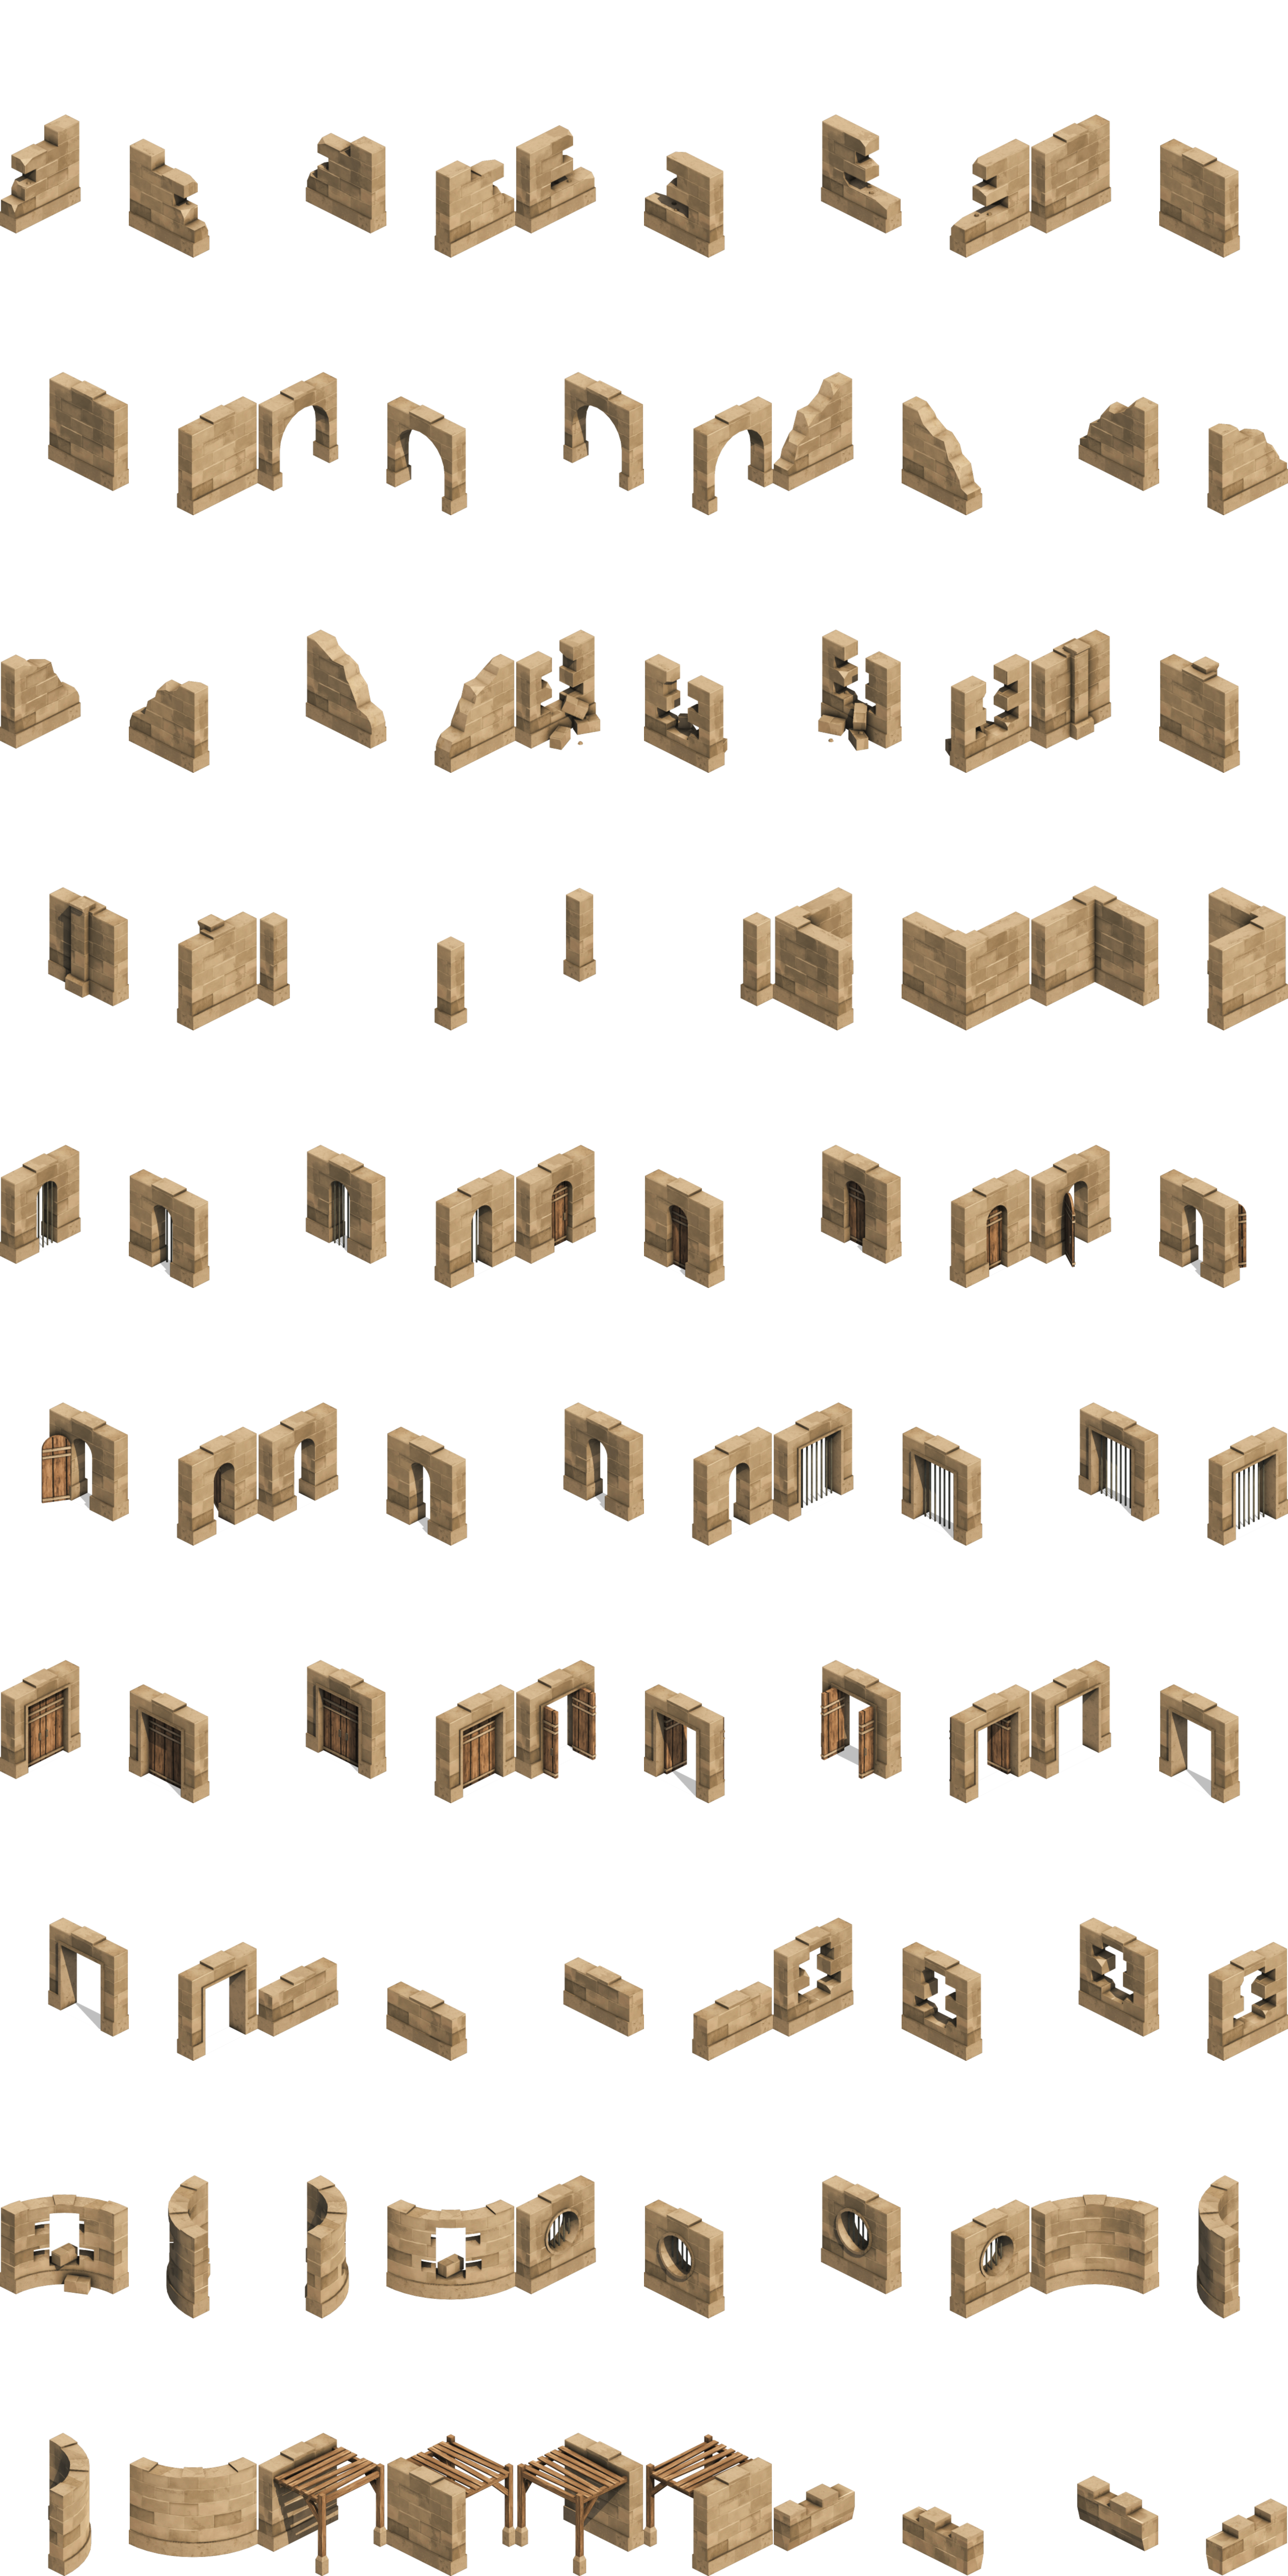
\includegraphics[width=0.65\textwidth]{images/all_100.png}
    \end{center}

    \newpage
    \item Table 200
    
    \begin{center}
    \includegraphics[width=0.65\textwidth]{images/all_200.png}
    \end{center}

    \newpage
    \item Table 300
    
    \begin{center}
    \includegraphics[width=0.65\textwidth]{images/all_300.png}
    \end{center}

    \newpage
    \item Table 400
    
    \begin{center}
    \includegraphics[width=0.65\textwidth]{images/all_400.png}
    \end{center}

    \newpage
    \item Table 500
    
    \begin{center}
    \includegraphics[width=0.65\textwidth]{images/all_500.png}
    \end{center}

\end{itemize}

\end{document}
